\section{Introduction to Systems Programming}

\subsection{What is Systems Software?}

Important aspects of systems software:

Systems software ...

\begin{itemize}
    \item ... closely interacts with the hardware.
    \item ... is concerned about efficiency.
    \item ... is used by other software as opposed to application software which is used by the end-user directly.
\end{itemize}

Examples for systems software:

\begin{itemize}
    \item Operating system
    \item Compiler
    \item Game engine
    \item Search engine
    \item Programming languages virtual machines e.g. java virtual machine
    \item Device drivers
    \item Any kind of server
\end{itemize}

Examples for application software:

\begin{itemize}
    \item Text editor
    \item Shopping website
    \item Social media apps
    \item Chat client
\end{itemize}

\subsection{Systems Programming Languages}

Systems programming languages are languages which make systems programming easy. There are three properties we are especially interested in:

\begin{enumerate}
    \item Direct access to hardware resources:
          \begin{itemize}
              \item Memory management
              \item Network throughput
              \item GPU
              \item CPU (single or multi core)
              \item threads and processes
          \end{itemize}
    \item Performance, therefore mostly compiled languages
    \item It would be nice to have some useful abstractions to improve productivity (C/C++ $\rightarrow$ Rust or Go).
\end{enumerate}

Examples for systems programming languages:

\begin{itemize}
    \item C, C++
    \item Rust
    \item Go
    \item Assembly (rarely)
\end{itemize}

Examples for application programming languages:

\begin{itemize}
    \item JavaScript (disgusted tone of voice)
    \item Python
    \item Java
\end{itemize}

\section{Memory Management and Memory Safety}

\subsection{Types of Memory}

Mainly the following types of memory exist in a computer ordered from small space and fast access speed to large space and slow access speed:

\begin{itemize}
    \item CPU registers
    \item Cache (L1, L2, L3)
    \item RAM
    \item SSD
    \item HDD
    \item Network Storage (Cloud, Backup)
\end{itemize}

\subsection{Locality}

There are two principles of locality which are used by caching algorithms:\\
\textbf{Spatial locality} assumes that after a certain portion of memory has been read, the next read memory addresses are  likely to be at a nearby memory address. This is true because of how e.g. arrays are designed and because of the fact that each process has an address space of consecutive memory addresses.
\textbf{Temporal locality} assumes that after a certain memory location has been read it is likely that it is going to be read again in a relatively short time span. This is true because of how logic computer programs usually works. If we read something from a location we often want to write something from that location and read it again shortly after.

\subsection{Virtual Memory}

There are two types of memory addresses: physical addresses and virtual addresses. Physical addresses are the addresses of bytes in RAM. Virtual memory addresses are addresses that are mapped to physical addresses. The virtual memory address space is much larger than the physical address space (RAM size) which allows us to use more memory than actually available. The mapping between virtual and physical memory is stored in a data structure called page table. The reason for using pages instead of a byte to byte mapping is that the page table would be way to large if we did so. In practice pages are e.g. 4KiB on unix systems.\\
Whenever the CPU executes a load or store instruction the virtual address first has to be resolved. in case the virtual address maps to a physical address in RAM the instruction can be executed right away. In case the virtual address is occupied but maps to a physical address on disc, which is called \textit{page fault}, the following things must happen:

\begin{itemize}
    \item An unused physical address must be found. If all physical addresses are occupied one page must be swaped out of RAM and stored on disc which is called \textit{page eviction}.
    \item The contents of the desired virtual memory address must be copied to RAM and the page table must be updated.
    \item The CPU instruction must be run again and will now not trigger a page fault.
\end{itemize}

\begin{figure}[h]
    \centering
    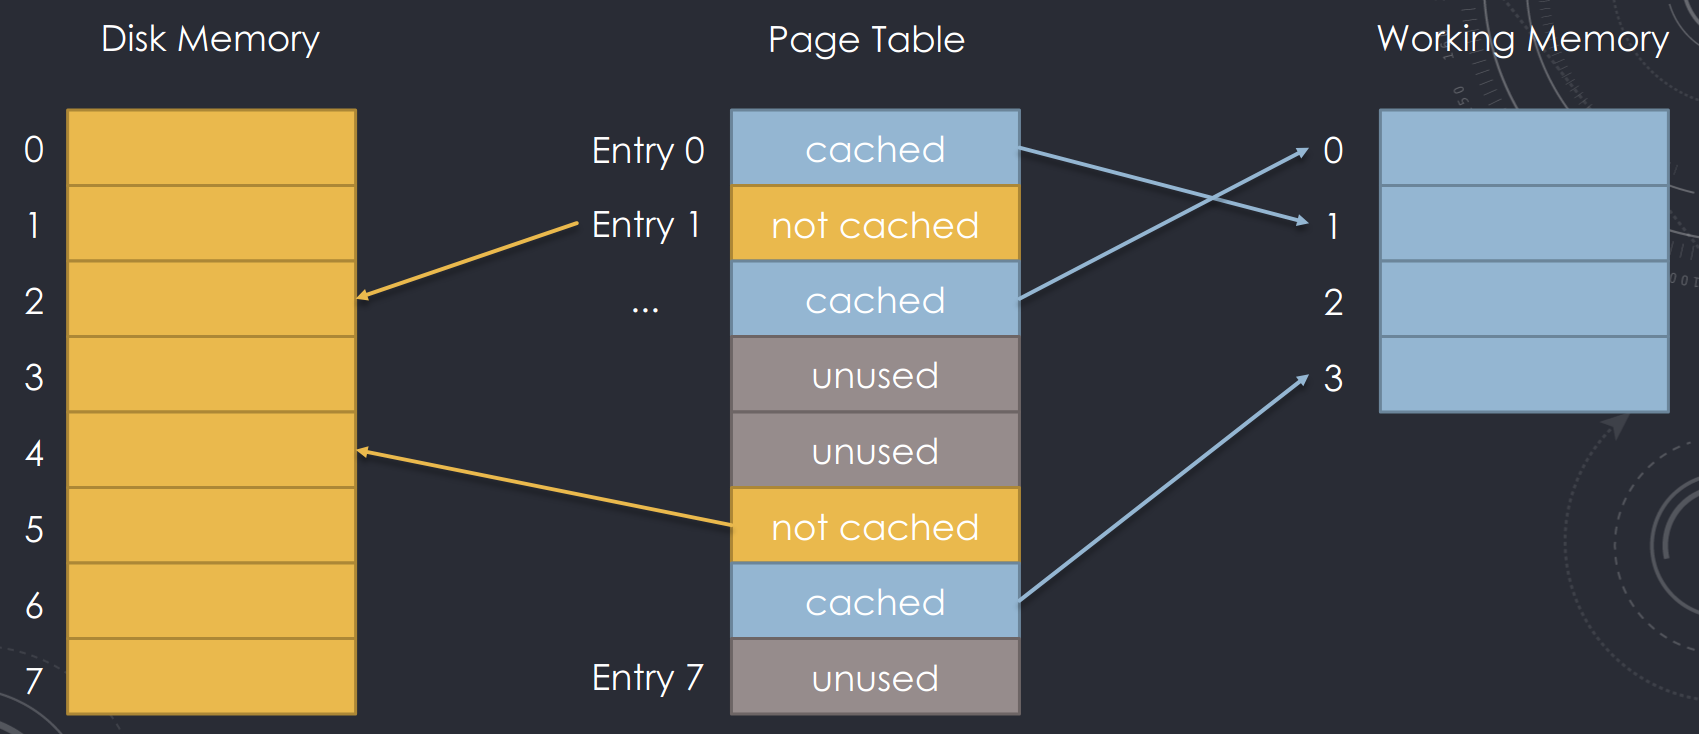
\includegraphics[width=500px]{virtual_mem_1.png}
    \caption{Visualization of virtual memory}
    \label{fig:virtual_memory}
\end{figure}

A virtual address is split into two parts: the page number (yellow) and the offset within the page (orange). With an address like shown in figure \ref{fig:virtual_memory_address} we can therefore address $2^{4} = 16$ virtual pages of the size of $2^{12} bit= 2^{2} \cdot 2^{10} bit = 4 KiB$.

            \begin{figure}[h]
                \centering
                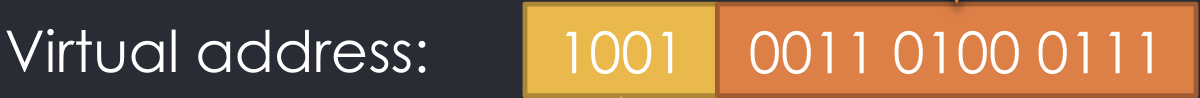
\includegraphics[width=300px]{virtual_memory_address.png}
                \caption{A single virtual address with page number in yellow and offset within page in orange}
                \label{fig:virtual_memory_address}
            \end{figure}

            A page table entry as shown in figure \ref{fig:page_table_entry} must then map the virtual page number (VPN) to a physical page number (PPN). As physical and virtual pages are of the same size the virtual page offset (VPO) and the physical page offset (PPO) are identical and must not be mapped. When mapping a virtual to a physical address like shown in figure \ref{fig:virtual_address_mapping} therefore first the cached flag (yellow) is checked. If it is equal to zero a page fault has occurred and the physical address must first be loaded into RAM and then the page table must be updated. Now the physical address is build by replacing the virtual page number (VPN) with the physical page number (PPN) in the virtual address.

            \begin{figure}[h]
                \centering
                
\includegraphics[width=300px]{page_table_entry.png}
                \caption{One page table entry with cached flag (yellow), virtual page number VPN (gray) and physical page number PPN (green)}
                \label{fig:page_table_entry}
            \end{figure}

            \begin{figure}[h]
                \centering
                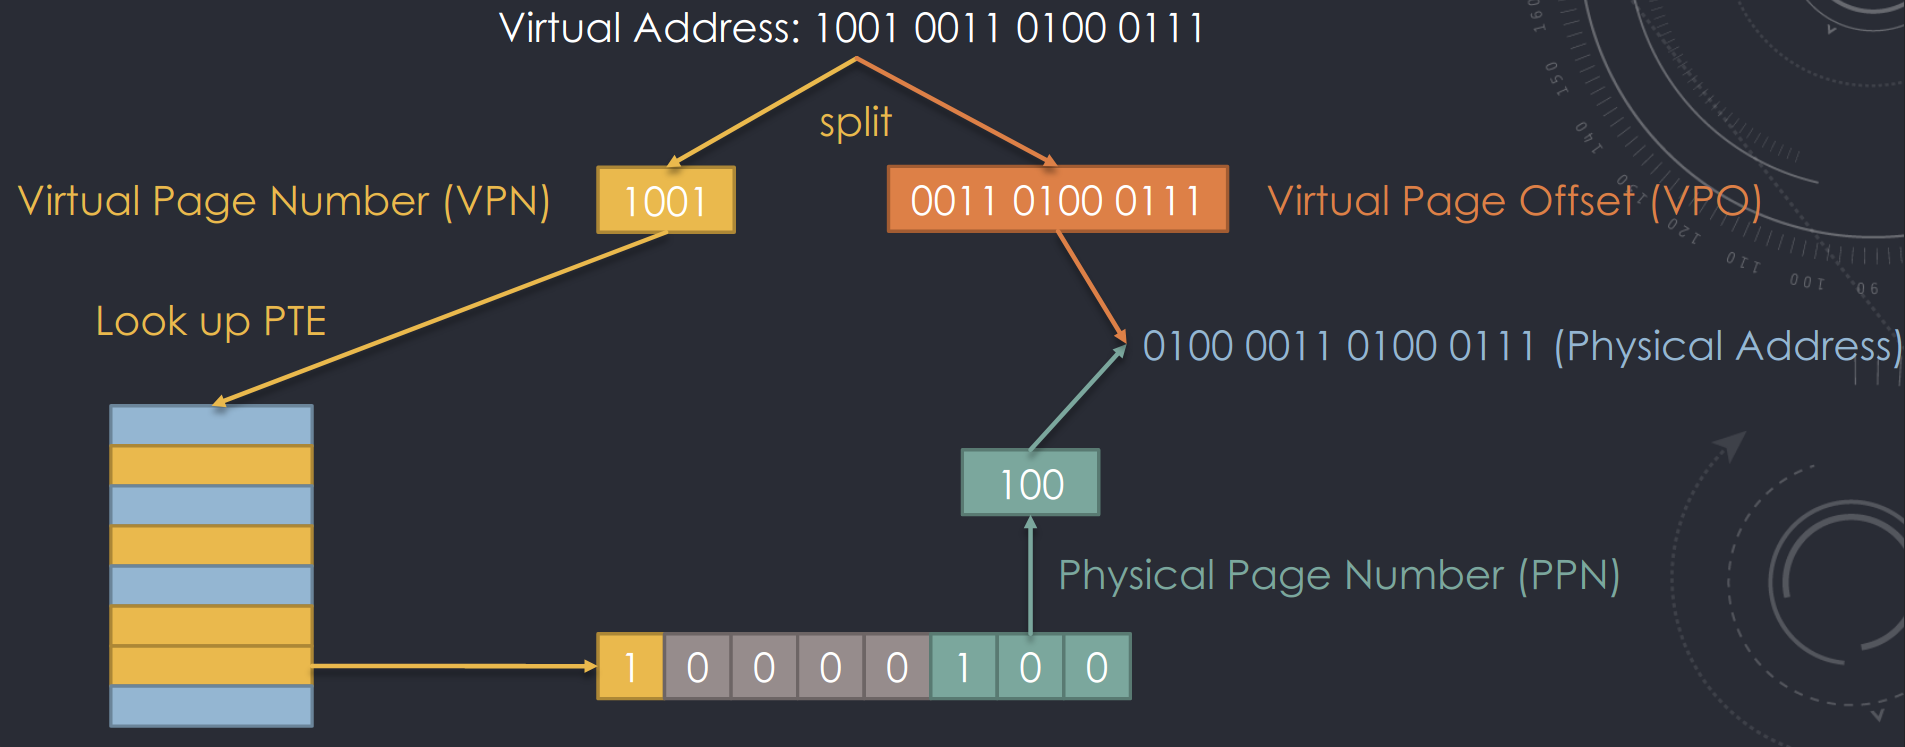
\includegraphics[width=500px]{virtual_address_mapping.png}
                \caption{Visualization of the process of mapping a virtual address to a physical address}
                \label{fig:virtual_address_mapping}
            \end{figure}


            \subsection{Return Value Optimization (RVO)}

            A common thing to do in C++ is to return a local variable from a function and assign it to a local variable of the calling function like shown in figure \ref{fig:rvo}. In this example if we assume we return a stack variable from the function \lstinline{add()}. Then if we resolve function calls we would end up with a local variable on the stack of the \lstinline{add()} function wich is written to the register R0 as a return value. Then the return value is copied into the variable \lstinline{result} by the \lstinline{main()} function. To prevent this unnecessary copying of stack variables the compiler in C++ is allowed to apply \textit{return value optimization (RVO)} and alter the normal behavior of stack cleanup to avoid the copying.

    \begin{figure}[h]
        \begin{lstlisting}
        int main(){
            int result = add(2, 2);
        }
    \end{lstlisting}
        \caption{Use case for return value optimization in C++}
        \label{fig:rvo}
    \end{figure}

    \subsection{Resource Acquisition is Initialization (RAII)}

    C++ introduced a term called RAII which stands for \textit{resource acquisition is initialization}. This refers to the behavior that if we use the \lstinline{new}-operator to allocate memory on the heap, we also automatically call a constructor which will initialize that memory for us. Also when freeing that memory location with the \lstinline{delete}-operator the destructor of the object is called to perform necessary cleanups. In pure C that was different as \lstinline{malloc} and \lstinline{free} do not initialize and cleanup their memory location. RAII is useful, can prevent frequent bugs and is of course also used in Rust.

    \subsection{Single Owner and Shared Owner Memory Management}

    In a single owner memory model like a \lstinline{vector} the object allocates memory once it is created and cleans it up once it goes out of scope. However with a shared memory management an object allocates the memory only if it is the first instance being created for a specific memory segment and only cleans up if it is the last object pointing to that memory segment. This behavior allows multiple owners of heap memory and prevents \textit{double free errors}. To be able to achieve this we need smart pointers with reference counting i.e. pointer types that check in their destructor if they are the last instance pointing to specific address.

    \subsection{Heap Containers in Rust}

    In figure \ref{fig:heap_containers_rust} a short summary of containers and types is shown to work with the heap in rust. Furthermore I would like to give some more details to the individual containers here:

    \begin{itemize}
        \item \lstinline{Rc<T>}: is a reference counting pointer. Its construction allocates memory on the heap. Using clone creates another instance of \lstinline{Rc<T>} pointing to the same memory location. Once the last instance of \lstinline{Rc<T>} pointing to that location goes out of scope it triggers the Drop trait for \lstinline{T}.
        \item \lstinline{Weak<T>}: is a pointer to a memory location which does not guarantee that memory location is still valid. It can be obtained via \lstinline{Rc::downgrade} and be converted to an \lstinline{Rc<T>} by calling \lstinline{upgrade}. When a \lstinline{Weak<T>} gets out of scope it never triggers the Drop Trait of \lstinline{T}. Also when all \lstinline{Rc<T>} pointing to one instance of T have been dropped \lstinline{Weak<T>}s to that location will return \lstinline{None} on \lstinline{upgrade} as they point to freed memory locations. \lstinline{Weak<T>} is useful to avoid circular dependencies between \lstinline{Rc}s.
        \item \lstinline{Cell<T>}: allows multiple owners of the same data. However, when retrieving that value the value will be copied. Therefore if we retrieve the value mutably inside the \lstinline{Cell<T>} twice in the same scope, this is possible, but also results in two independent variables.
        \item \lstinline{RefCell<T>}: allows multiple mutable owners of the same data. When retrieving a reference to the inner value it is checked that there is currently no other access to the inner value, otherwise the \lstinline{borrow_mut} function panics. This way the borrow checking rules are enforced at runtime. This means we will never have two mutable references to the same data at the same time, because we otherwise panic. The programmer must now make sure he will not get a panic. This is not thread safe.
        \item \lstinline{Arc<T>}: is an atomic reference counting pointer. It can be used across threads in order to have multiple threads accessing the same data. However it requires the wrapped value to be Sync, which means it must also be thread safe to access that. This can be ensured by wrapping the inner value inside of a \lstinline{Mutex<T>} or a \lstinline{RwLock<T>}.
    \end{itemize}

    \begin{figure}[h]
        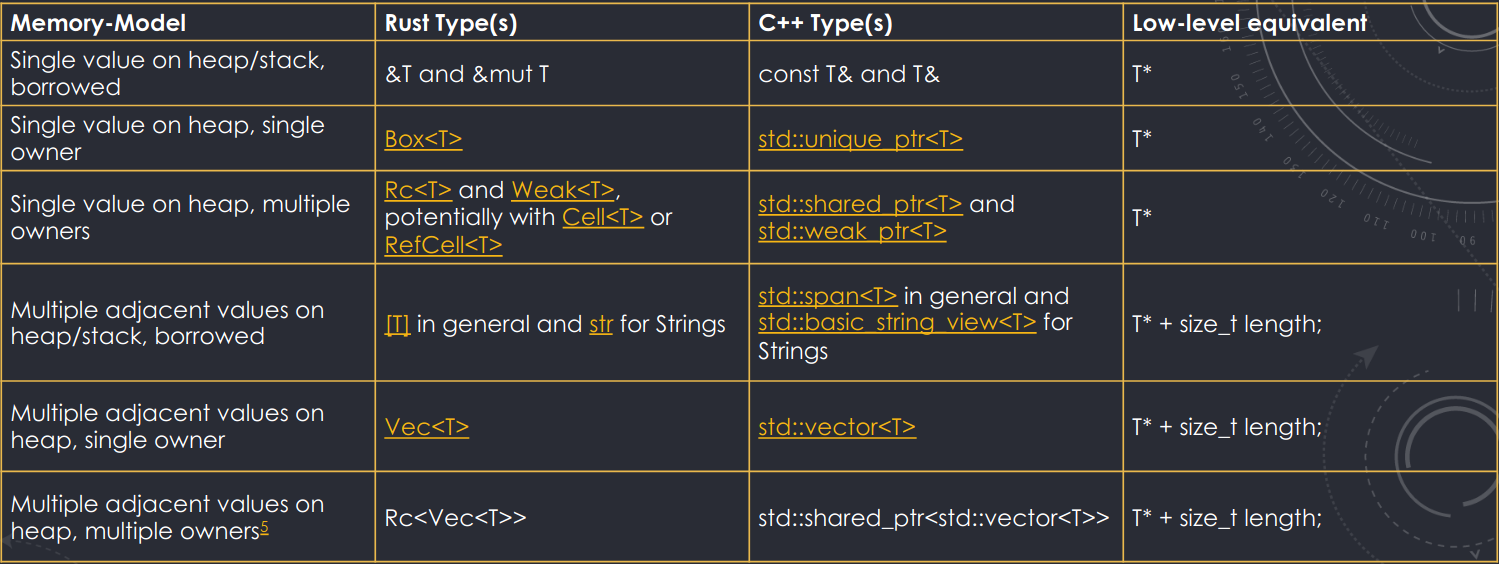
\includegraphics[width=500px]{memory_cheat_sheet.png}
        \caption{Use case for return value optimization in C++}
        \label{fig:heap_containers_rust}
    \end{figure}


    \section{Zero Overhead Abstractions}

    Zero Overhead abstractions are abstractions that have no performance overhead at runtime compared to the most optimal handwritten solution for the problem.

    \subsection{Product Types and Sum Types}

    Each primitive type has a finite set of possible values it can take on. However, we can define product types and sum types that build an abstraction on top of primitive types.\\
    Product types are types whose set of possible values is of the size of the product of the amount of possible values of all contained types, an example are structs or classes.\\
    Sum types are types whose size of the set of possible values is the sum of the amount of distinct values of all contained types, an example are rust enums.

    \subsection{Iterators}

    Iteration can be defined as a sequence of the following three operations:

    \begin{itemize}
        \item Dereferencing: Get access to current element
        \item Incrementing: Move to next element
        \item Comparing: Check if we are at the end of collection
    \end{itemize}

    In Rust all these three properties are usable with only one method which is called \lstinline{next()}. It retrieves the current element if there is one, otherwise returns \lstinline{None} and increments the iterator.

    In contrast to C++, rust uses stateful iterators, which means that the iterator knows its current position inside a collection and will return \lstinline{None} once it has reached the end.

    \subsection{Algorithms}

    In the following we will summarize some of the useful algorithms that are supplied for working with rust iterators:

    \begin{enumerate}
        \item \lstinline{all}: returns true if all elements meet a certain condition
        \item \lstinline{any}: returns true if at least one element meets a certain condition
        \item \lstinline{is_partitioned}: returns true if there is a boundary in the container such that all elements before the boundary are either true or false and after the boundary the oposite.
        \item \lstinline{filter}: Returns an iterator over all elements that meet a given condition.
        \item \lstinline{filter_map}: returns an iterator over all elements of Type U for which a filter closure returns Some(U)
        \item \lstinline{position}: returns the Some(index) of the first element matching a condition
        \item \lstinline{find}: returns Some(T) for the first element of type T matching a condition.
        \item \lstinline{collect}: returns a collection storing all elements over which has been iterated
        \item \lstinline{count}: Returns the number of elements over which is being iterated.
        \item \lstinline{for_each}: calls a function without return value taking each element as an input.
        \item \lstinline{max}: returns the maximum element
        \item \lstinline{min}: returns the minimum element
        \item \lstinline{fold}: takes a start value of Type U and a closure with 2 parameters T and U with return value U which will be called for each element. Returns a value of type U which is the result of calling the closure with the accumulated value and the current value of the iterator for each element.
        \item \lstinline{reduce}: Combines two elements of type T to one repeating this for each element and returning the resulting scalar value T.
        \item \lstinline{sum}: fold with start value 0 and an addition as closure.
        \item \lstinline{product}: fold with start value 1 and multiplication as closure.
        \item \lstinline{step(n)}: returns an element over every n-th element
        \item \lstinline{peekable}: returns a peekable iterator which is an iterator which can call .peek() which means returning the current element without incrementing the position.
        \item \lstinline{map}: converts each element of type T into an element of type U by calling a closure.
        \item \lstinline{flatten}: converts an iterator over iterators (nested iterator) into an iterator over elements of the inner type (like flattening a 2d-array to a 1d array).
        \item \lstinline{intersperse(val)}: returns an iterator over the elements separated by the given val.
        \item \lstinline{cycle}: returns a never ending iterator that returns the elements of the given iterator in a cycle.
        \item \lstinline{chain(other)}: concats iterators
        \item \lstinline{enumerate}: returns an iterator over tuples of (index, element).
        \item \lstinline{fuse}: returns an iterator that will always return None after having returned None once on calling \lstinline{next}.
        \item \lstinline{rev}: returns an iterator over the elements in reversed order
        \item \lstinline{zip(other)}: returns an iterator over tuples of the elements of both iterators.
    \end{enumerate}

    Note that rust iterators are online iterators, which means they work with one piece of data at a time and therefore do not support sorting, however collections in rust often have sort methods.

    \section{Error Handling}

    There are three common ways of error handling:

    \begin{itemize}
        \item Error Codes like in C:
              \begin{itemize}
                  \item[+] easy and not complicated
                  \item[-] abuse of return type makes certain values unusable for non-error cases
                  \item[-] easy to ignore errors returned by a function
                  \item[-] error codes have no names and must be transated using documentation
                  \item[-] specific error data must be read from global variables
              \end{itemize}
        \item Exceptions like in C++:
              \begin{itemize}
                  \item[+] convenient for user as the function call is separated from the catch statement
                  \item[-] not transparent which function throws what errors
              \end{itemize}
        \item Result Type like in Rust:
              \begin{itemize}
                  \item[+] error must be handled explicitly
                  \item[+] errors can deliver error details to the caller
                  \item[+] it is clear to the caller what error can be returned by e.g. using an enum as error type inside a result type.
              \end{itemize}
    \end{itemize}


    \section{Systems Level I/O}

    \subsection{Files}

    \textit{A file is a sequence of bytes}. It can be stored persistently on disc or also just in memory. Unix was build on the idea that the following operations are everything needed to work with files:

    \begin{itemize}
        \item Opening
        \item Closing
        \item Changing position inside a file
        \item Reading a range of bytes from current position
        \item Writing a range of bytes to current position
    \end{itemize}

    In unix all types of input and output are modeled using files such as:
    \begin{itemize}
        \item Reading from and writing to disk
        \item Reading from and writing to network streams
        \item Reading from and writing to the terminal
    \end{itemize}

    \subsection{Interprocess Communication}

    Two types of communication:

    \begin{enumerate}
        \item Process control: with Signals
              \begin{itemize}
                  \item Signals inform processes about low level system events having happened and are handles using a signal handler
                  \item Signals can be send using the \textit{kill} command
                  \item signals are basically just an integer encoding an event, they have no payload -> not suitable for information exchange
              \end{itemize}
        \item Information exchange: with I/0 or shared Memory
              \begin{itemize}
                  \item We can share some pages of memory between processes with the \textit{mmap} function in C.
                  \item Shared memory fast but difficult and most of the time inconvenient
                  \item Standard way is using I/O such as TCP streams
              \end{itemize}
    \end{enumerate}

    \subsubsection*{Command Line Arguments}

    In rust we can access the command line arguments using \lstinline{st::env::args()} which returns an iterator over all cli arguments.

    \subsubsection*{Environment Variables}

    Environment variables are key value pairs that can be set on the operating system for one process. There are some predefined variables. When using \lstinline{int execve(const char *filename, char *const argv[], char *const envp[]);} to spawn a new process, the environment variables of the parent process are passed to the child process via the third argument to it's main function \lstinline{int main(int argc, char *argv[], char *envp[])}

    \section{Fearless Concurrency with Rust}

    \subsection{Ways of Parallelism}

    \begin{enumerate}
        \item Instruction Level Parallelism: Pipelining
        \item Hyperthreading: Duplicating certain parts like the ALU inside a single processor to run multiple instructions at once. This is possible because one instruction may only need some parts of the CPU and another instruction may need other parts of the CPU.
        \item SIMD: perform same operation on multiple words -> data level parallelism
        \item Using multiple Cores with multithreading or multiple processes.
    \end{enumerate}

    \subsubsection*{Threads in Rust}

    Via the interface \lstinline{std::thread::spawn(FnOnce + Send) -> JoinsHandle<T>} we can start a new thread executing a closure which will return a join handle. Join handles are used to join or detach threads later on. All variables captured in the closure must be owned by it i.e. must be moved into the closure using \lstinline{std::thread::spawn(move || ...}.

    \subsection{The Fork Join Pattern}

    The fork join pattern says that a task can be parallelized by first splitting the task into $n$ disjunct sub tasks by the master thread, then spawning $n-1$ worker threads and executing the tasks and eventually merging the result into one single result by the master thread again.

\subsection{The rayon parallelism crate}

Rayon provides parallel iterators which are very easy to use and can parallelize tasks on big containers:

\begin{lstlisting}
    fn search_parallel_rayon(text: &str, keyword: &str, parallelism: usize) -> usize {
    let chunks = chunk_string_at_whitespace(text, parallelism);
    chunks
        .par_iter()
        .map(|chunk| search_sequential(chunk, keyword))
        .sum()
    }
\end{lstlisting}

\subsection{Asynchronous I/O}

Threads are great for saturating the CPU with a lot of work. But if we have many small tasks then it might be better to use asynchronous programming. The challenge that asynchronous code comes to solve is how to handle multiple streams of tasks at the same time when using one thread per task is not suitable because most of the times the threads would wait for tasks. I.e. how to handle multiple connections where most of the time on each connection is spend waiting for a message. This comes eventually down to the idea that we observe a pool of actions often called Futures with only one thread and want to make sure we always handle the first Future that is ready and execute the corresponding code. This can be implemented with interfaces like \lstinline{poll} in C, however, is not very convenient. Asynchronous patterns in rust with async and await add a layer of abstraction on top of that. We can define that a function is async which means it returns a Future which can be awaited. Because async functions can only be called inside of other async functions that comes down to the main function being async. Then we need some kind of executor which is essentially a runtime to execute our async main function. Executors are supplied by libraries like tokio. The executor then calls await on the outer most future which will call poll on all futures until one of the polls returns Poll::Pending. This call also schedules a waker which will notify the executor when the future has new data and shall be polled again.